\documentclass[11pt]{article}
\usepackage[a4paper,margin=2.5cm]{geometry}
\usepackage{amsmath,amssymb,amsthm,graphicx,booktabs,xcolor}
\usepackage[colorlinks=true,linkcolor=blue!60!black,citecolor=blue!60!black,urlcolor=blue!60!black]{hyperref}
\usepackage{xurl}
\hypersetup{pdftitle={Closing the Tsirelson Loophole in Relativistic Quantum Field Theory},pdfauthor={Ruqing Chen}}
\setlength{\emergencystretch}{3em}
\graphicspath{{../figures/}{figures/}{./}}

\newtheorem{theorem}{Theorem}
\newtheorem{proposition}{Proposition}[section]
\newtheorem{corollary}{Corollary}[section]
\newtheorem{lemma}{Lemma}[section]
\theoremstyle{definition}\newtheorem{definition}{Definition}[section]
\theoremstyle{remark}\newtheorem*{remark}{Remark}

\newcommand{\dd}{\mathrm{d}}
\newcommand{\Hil}{\mathcal H}
\newcommand{\A}{\mathcal A}
\newcommand{\M}{\mathcal M}
\newcommand{\N}{\mathcal N}
\newcommand{\Cqa}{C_{qa}}
\newcommand{\Cqs}{C_{qs}}
\newcommand{\Cqc}{C_{qc}}
\newcommand{\paperdoi}{10.5281/zenodo.23202937}

\title{Closing the Tsirelson Loophole\\ in Relativistic Quantum Field Theory:\\
Split Inclusions, Hyperfinite Local Algebras,\\ and the Effective Dimension of the Vacuum}
\author{Ruqing Chen\\[2pt]
\small GUT Geoservice Inc., Montreal, Quebec, Canada\\
\small \href{mailto:ruqing@hotmail.com}{\texttt{ruqing@hotmail.com}}}
\date{\small DOI: \href{https://doi.org/\paperdoi}{\paperdoi}}

\begin{document}
\maketitle

\begin{abstract}
MIP$^*$=RE implies that correlations of commuting observables on an infinite-dimensional Hilbert space can lie at a
finite distance from every limit of finite-dimensional tensor-product correlations. Such correlations would let a
finite experiment detect an actual infinity with a modest number of rounds. In earlier work we identified this as the
only route that escapes the resource bounds on certifying Hilbert-space dimension. Here we ask whether relativistic
quantum field theory allows Bell correlations in this gap.

The answer is no under standard structural assumptions. If the theory has the split property, which follows from the
Buchholz--Wichmann nuclearity condition and holds for free fields, then the correlations of local measurements in
strictly spacelike separated regions are tensor-product correlations and lie in $\Cqa$. If the local algebras are
hyperfinite, as Buchholz, D'Antoni and Fredenhagen showed under a scaling-limit assumption, the same holds for regions
that are merely spacelike, with no gap between them. We give a self-contained proof of the second statement from
semidiscreteness. Alice's measurements are compressed through matrix algebras by unital completely positive maps, and
the resulting correlations converge to the original ones. The static-patch algebra of de Sitter space constructed by
Chandrasekaran, Longo, Penington and Witten is a corner of a crossed product of such an algebra by $\mathbb R$, so it is
again injective. Thus, in these frameworks, the gap found by MIP$^*$=RE cannot be realised by local measurements.

We then bound how much dimension a Bell test can certify from the state side. Compressing each party to the support of
its $\varepsilon$-smoothed reduced state reproduces all correlations to within $2(\sqrt{\varepsilon_A}+\sqrt{\varepsilon_B})+\varepsilon_A+\varepsilon_B$. An experiment
with $N$ rounds can therefore certify at most the smooth max-entropy of the local state at smoothing $\varepsilon\sim1/N$. For
the vacuum of a lattice free scalar field we compute this effective dimension exactly. It follows an area law, at
most $9$ bits for a $128$-site block at $\varepsilon=10^{-6}$ against $553$ bits from naive counting. It grows only from $2.3$ to
$13.1$ bits as $\varepsilon$ decreases from $10^{-1}$ to $10^{-12}$, with a local slope that falls from $0.60$ to $0.19$ bits per bit of
precision. A product bound over thermal modes shows that the growth is polylogarithmic in $1/\varepsilon$ for any regularised block.
\end{abstract}

\tableofcontents

%=====================================================================
\section{Introduction}
\label{sec:intro}

Bell experiments are usually modelled in two ways. In the tensor-product model, Alice and Bob act on the factors of
$\Hil_A\otimes\Hil_B$. In the commuting-operator model, which is the natural framework of algebraic quantum field
theory~\cite{Haag}, their observables act on a single Hilbert space and merely commute. Let $C_q$ denote the
correlations of finite-dimensional tensor-product strategies, $\Cqa$ its closure, $\Cqs$ the correlations of possibly
infinite-dimensional tensor-product strategies, and $\Cqc$ the commuting-operator correlations. Then
$C_q\subseteq\Cqs\subseteq\Cqa\subseteq\Cqc$~\cite{ScholzWerner,Fritz}. Tsirelson's problem asked whether $\Cqa=\Cqc$. It is
equivalent to Connes' embedding problem~\cite{JungeEtAl,Fritz}, and MIP$^*$=RE answered both in the negative~\cite{MIPRE}.

The answer matters for the question of whether an actual infinity is empirically accessible. In a companion
paper~\cite{Chen2026_certify} we showed that certifying a Hilbert-space dimension beyond holographic bounds with known
dimension witnesses requires more experimental rounds than the region can perform. The single exception is the gap
between $\Cqa$ and $\Cqc$. A correlation in $\Cqc\setminus\Cqa$ has a finite distance from every finite-dimensional model, so a
finite number of rounds could exhibit it. Cabello, Quintino and Kleinmann listed four logical possibilities for the
physical status of such correlations, ranging from ``never realisable'' to ``realisable by spacelike separated
parties''~\cite{CabelloQuintinoKleinmann}. They mention the split property and the role of nuclear algebras, but they do
not draw a conclusion for quantum field theory.

We show that standard structural results of algebraic QFT settle the question for local measurements.
\begin{itemize}
\item \emph{Split inclusions} (Theorem~\ref{thm:split}). If Alice's region has a neighbourhood that is still spacelike
to Bob's region, the split property makes the correlations tensor-product correlations. They lie in $\Cqs\subseteq\Cqa$.
\item \emph{Hyperfinite local algebras} (Theorem~\ref{thm:injective}). If Alice's local von Neumann algebra is injective,
equivalently hyperfinite, every correlation with commuting partners lies in $\Cqa$, even without a gap between the
regions.
\item \emph{de Sitter space} (Proposition~\ref{prop:dS}). The type II$_1$ algebra of an observer in a de Sitter static
patch is injective under the same assumptions.
\item \emph{Effective dimension} (Section~\ref{sec:effective}). An $N$-round Bell test certifies at most the smooth max-entropy
of the local state at smoothing $\varepsilon\sim1/N$. For the vacuum of a lattice free field this is small, follows an area law
and grows polylogarithmically in $1/\varepsilon$.
\end{itemize}

%=====================================================================
\section{Correlation sets and local algebras}
\label{sec:setting}

A Bell scenario has finitely many settings $x,y$ and outcomes $a,b$. A commuting-operator strategy consists of a
Hilbert space $\Hil$, a normal state $\omega$ on $B(\Hil)$, and POVMs $\{A^x_a\}$, $\{B^y_b\}$ with $[A^x_a,B^y_b]=0$. The
correlation is $p(a,b|x,y)=\omega(A^x_aB^y_b)$. We use two standard facts.

\begin{lemma}[\cite{ScholzWerner,Fritz}]
\label{lem:qs}
$\Cqs\subseteq\Cqa$: correlations of tensor-product strategies on infinite-dimensional spaces are limits of
finite-dimensional ones.
\end{lemma}

\begin{lemma}
\label{lem:finiteA}
If Alice's POVM elements lie in a finite-dimensional C$^*$-algebra $F$, and Bob's commute with $F$, then the correlation lies
in $\Cqs$.
\end{lemma}

\begin{proof}
A unital representation of $F\cong\bigoplus_kM_{n_k}$ decomposes $\Hil=\bigoplus_k\mathbb C^{n_k}\otimes\mathcal K_k$, with $F$ acting as
$\bigoplus_kX_k\otimes1$ and with commutant $\bigoplus_k1\otimes B(\mathcal K_k)$. Hence Alice's operators have the form $\bigoplus_kX_k\otimes1$ and
Bob's the form $\bigoplus_k1\otimes Y_k$. The subspace $\bigoplus_k\mathbb C^{n_k}\otimes\mathcal K_k$ embeds isometrically into
$\bigl(\bigoplus_k\mathbb C^{n_k}\bigr)\otimes\bigl(\bigoplus_k\mathcal K_k\bigr)$, where $\bigoplus_kX_k$ and $\bigoplus_kY_k$ act on the two factors and agree with
the original operators on the image. The state is supported on the image, so the correlation is unchanged and lies in
$\Cqs$.
\end{proof}

\paragraph{Local quantum physics.} A net $O\mapsto\A(O)$ assigns von Neumann algebras on the vacuum Hilbert space to
regions of Minkowski space, with locality, $\A(O_1)\subseteq\A(O_2)'$ for spacelike separated regions~\cite{Haag}. A
local measurement in $O$ is a POVM with elements in $\A(O)$. Two structural properties are known to hold in large
classes of theories.
\begin{itemize}
\item \emph{Split property.} For $O\Subset\tilde O$ (the closure of $O$ lies in the interior of $\tilde O$) there is a type I
factor $\N$ with $\A(O)\subseteq\N\subseteq\A(\tilde O)$~\cite{DoplicherLongo}. It follows from the Buchholz--Wichmann
nuclearity condition, which bounds the energy-level density of localised states, and holds for free
fields~\cite{BuchholzWichmann}.
\item \emph{Hyperfiniteness.} Under the standard postulates and the existence of a scaling limit, each local algebra is
isomorphic to $\mathcal R\otimes\mathcal Z$, where $\mathcal R$ is the unique hyperfinite factor of type III$_1$~\cite{Haagerup}
and $\mathcal Z$ is the centre~\cite{BDF}. In particular local algebras are injective.
\end{itemize}

%=====================================================================
\section{Local measurements cannot reach the Tsirelson gap}
\label{sec:theorems}

\begin{theorem}[Split inclusions]
\label{thm:split}
Let $O_A\Subset\tilde O_A$ and let $O_B$ be spacelike to $\tilde O_A$. If the split property holds for $O_A\subseteq\tilde O_A$, then for
every normal state and all local measurements in $O_A$ and $O_B$ the correlation lies in $\Cqs\subseteq\Cqa$.
\end{theorem}

\begin{proof}
Let $\N$ be a type I factor with $\A(O_A)\subseteq\N\subseteq\A(\tilde O_A)$. Locality gives $\A(O_B)\subseteq\A(\tilde O_A)'\subseteq\N'$. A type I
factor induces a tensor factorisation $\Hil\cong\mathcal K_1\otimes\mathcal K_2$ with $\N=B(\mathcal K_1)\otimes1$ and $\N'=1\otimes B(\mathcal K_2)$. Alice's
POVM elements lie in $B(\mathcal K_1)\otimes1$, Bob's in $1\otimes B(\mathcal K_2)$, and the state is a density operator on $\mathcal K_1\otimes\mathcal K_2$.
The correlation is therefore in $\Cqs$, and Lemma~\ref{lem:qs} gives $\Cqa$.
\end{proof}

For regions without a gap, for example complementary wedges, a type I factor between them does not exist. Injectivity
replaces it. Recall that a von Neumann algebra $\M$ is \emph{semidiscrete} if there are nets of normal unital completely
positive (ucp) maps $\alpha_k:\M\to M_{n_k}$ and $\beta_k:M_{n_k}\to\M$ with $\beta_k\circ\alpha_k\to\mathrm{id}_\M$ pointwise in the
$\sigma$-weak topology. Semidiscreteness is equivalent to injectivity and to hyperfiniteness~\cite{Connes,EffrosLance}.

\begin{theorem}[Injective local algebras]
\label{thm:injective}
Let $\M\subseteq B(\Hil)$ be an injective von Neumann algebra, $\omega$ a normal state, $\{A^x_a\}\subseteq\M$ Alice's POVMs and
$\{B^y_b\}\subseteq\M'$ Bob's POVMs. Then $p(a,b|x,y)=\omega(A^x_aB^y_b)$ lies in $\Cqa$.
\end{theorem}

\begin{proof}
Take $\alpha_k,\beta_k$ as above. Since $M_{n_k}$ is finite-dimensional, hence nuclear, the algebraic tensor product
$M_{n_k}\odot\M'$ carries a unique C$^*$-norm, and we write $M_{n_k}\otimes\M'$ for its completion. Since $\beta_k:M_{n_k}\to\M$ is
completely positive and its range commutes with $\M'$, the map $X\otimes Y\mapsto\beta_k(X)Y$ extends to a completely positive map on
$M_{n_k}\otimes\M'$~\cite{Paulsen}. Hence
$\varphi_k(X\otimes Y)=\omega(\beta_k(X)Y)$ is a state on $M_{n_k}\otimes\M'$. The operators $\tilde A^x_a=\alpha_k(A^x_a)$ form POVMs in $M_{n_k}$ because
$\alpha_k$ is ucp. Consider the strategy given by the GNS representation of $\varphi_k$, with Alice measuring $\tilde A^x_a$ and Bob
measuring $B^y_b$. Its correlation is
\begin{equation}
p_k(a,b|x,y)=\varphi_k(\tilde A^x_a\otimes B^y_b)=\omega\bigl(\beta_k(\alpha_k(A^x_a))\,B^y_b\bigr).
\end{equation}
Alice's algebra in this representation is the image of the finite-dimensional algebra $M_{n_k}$, so $p_k\in\Cqs$ by
Lemma~\ref{lem:finiteA}. As $k\to\infty$, $\beta_k\circ\alpha_k(A^x_a)\to A^x_a$ $\sigma$-weakly. Since $Z\mapsto\omega(ZB^y_b)$ is a normal functional,
$p_k\to p$. Thus $p$ lies in the closure of $\Cqs$, which is $\Cqa$ by Lemma~\ref{lem:qs}.
\end{proof}

\begin{remark}
Theorem~\ref{thm:injective} is the von Neumann-algebraic form of the known fact that $\Cqa$ and $\Cqc$ agree when one
party's algebra is nuclear~\cite{ScholzWerner,CabelloQuintinoKleinmann}. It is also closely related to the
tensor-product characterisations of semidiscreteness by Effros and Lance~\cite{EffrosLance}. We include the short proof because the compression maps $\alpha_k$ make the finite-dimensional
approximation explicit.
\end{remark}

\begin{corollary}
\label{cor:qft}
In a local net with hyperfinite local algebras, every Bell correlation between local measurements in spacelike
separated regions $O_A,O_B$ lies in $\Cqa$. If only the split property is known, the same holds whenever $O_A$ has a
neighbourhood spacelike to $O_B$. In either case no Bell functional separating $\Cqa$ from $\Cqc$ can be violated by local
measurements in spacelike separated regions. Among the four possibilities of~\cite{CabelloQuintinoKleinmann}, such
theories therefore exclude the fourth, in which correlations in $\Cqc\setminus\Cqa$ are realised by local observers in spacelike
separated regions. They
are silent on the second and third, which involve measurements on a single system or without spacelike separation.
\end{corollary}

\begin{proof}
Locality gives $\A(O_B)\subseteq\A(O_A)'$. Apply Theorem~\ref{thm:injective} with $\M=\A(O_A)$, or Theorem~\ref{thm:split}.
\end{proof}

\paragraph{de Sitter space.} Chandrasekaran, Longo, Penington and Witten constructed the algebra of observables
accessible to an observer in a static patch of de Sitter space, gravitationally dressed to the observer's
worldline~\cite{CLPW}. It is a von Neumann algebra of type II$_1$, obtained by projecting the crossed product of the
static-patch QFT algebra by its modular flow. It has a maximum-entropy state whose entropy agrees, up to a constant, with
the generalised entropy.

\begin{proposition}
\label{prop:dS}
If the static-patch QFT algebra is injective, as in the hyperfinite case above, then the de Sitter observer algebra
of~\cite{CLPW} is injective. Consequently all correlations between this observer and any party whose observables commute
with the observer's lie in $\Cqa$.
\end{proposition}

\begin{proof}
Crossed products of injective von Neumann algebras by actions of amenable locally compact groups, such as $\mathbb R$, are
injective, and so are corners $p\M p$ of injective algebras~\cite{BrownOzawa,Connes}. Apply Theorem~\ref{thm:injective}.
\end{proof}

%=====================================================================
\section{The effective dimension certified by a Bell test}
\label{sec:effective}

Theorems~\ref{thm:split} and~\ref{thm:injective} say that local QFT correlations can be approximated by finite-dimensional
ones. The next question is how large the approximating dimension must be at a given precision. For a density operator
$\rho$, let $d_\rho(\varepsilon)$ be the smallest rank of a projector $P$ with $\mathrm{tr}(P\rho)\ge1-\varepsilon$, so that
$\log_2d_\rho(\varepsilon)$ is the smooth max-entropy $H_0^\varepsilon(\rho)$~\cite{RennerWolf}.

\begin{proposition}
\label{prop:compress}
Let $\rho_{AB}$ be a state on $\Hil_A\otimes\Hil_B$ with marginals $\rho_A,\rho_B$, and let $\varepsilon_A,\varepsilon_B\in(0,1)$. There is a state supported on a
subspace of local dimensions $d_{\rho_A}(\varepsilon_A)$ and $d_{\rho_B}(\varepsilon_B)$ whose correlations, for all POVMs, differ from those of $\rho_{AB}$
by at most
\begin{equation}
\delta=2(\sqrt{\varepsilon_A}+\sqrt{\varepsilon_B})+\varepsilon_A+\varepsilon_B
\end{equation}
in total variation, for every pair of settings. Consequently, a test that certifies local dimension larger than
$\max(d_{\rho_A}(\varepsilon_A),d_{\rho_B}(\varepsilon_B))$ with error $\le\delta_0$ against $\rho_{AB}$ needs $N\gtrsim\ln(1/4\delta_0)/\delta^2$ rounds.
\end{proposition}

\begin{proof}
Let $P_A,P_B$ be the optimal projectors. By the gentle-measurement lemma~\cite{Winter},
$\|\rho_{AB}-(P_A\otimes1)\rho_{AB}(P_A\otimes1)\|_1\le2\sqrt{\varepsilon_A}$, and similarly for $B$. Normalising $\sigma=(P_A\otimes P_B)\rho_{AB}(P_A\otimes P_B)$ costs at
most $\varepsilon_A+\varepsilon_B$ in trace norm. On $\sigma$, a POVM $\{A_a\}$ acts as the compressed POVM $\{P_AA_aP_A\}$ on $P_A\Hil_A$. Trace distance
bounds the total-variation distance of all outcome distributions. The bound on $N$ follows from Theorem~1 of~\cite{Chen2026_certify}
with $\varepsilon_G$ replaced by $\delta$.
\end{proof}

The smoothing parameter enters quadratically. For $\varepsilon_A=\varepsilon_B=\varepsilon$ the gentle-measurement bound gives $\delta\approx4\sqrt\varepsilon$, while
$N$ independent rounds resolve $\delta\sim N^{-1/2}$. The relevant smoothing is therefore $\varepsilon\sim\delta^2/16\sim1/N$, not $N^{-1/2}$.

In QFT the reduced state on a local algebra is not a density operator, since the algebra is of type III. The split
property supplies one: the vacuum restricted to the type I factor $\N$ of Theorem~\ref{thm:split} is normal and has a density
operator. Proposition~\ref{prop:compress} applies to it, and the effective dimension depends on the size of the gap between
the regions. For a lattice regularisation the block is itself a type I system.

\begin{remark}[Continuum]
Among the intermediate type I factors there is a canonical one, constructed by Doplicher and Longo from the modular
conjugation of the relative commutant~\cite{DoplicherLongo}. The von Neumann entropy of the vacuum on it, the
canonical entanglement entropy, is finite for the chiral net of finitely many free fermions~\cite{LongoXu} and for a
broad class of conformal nets~\cite{PanebiancoWegener}. In the continuum limit it coincides with the reflected entropy
of the two regions~\cite{DuttaFaulkner}, which has been computed for the two-dimensional Dirac field as a function of the
cross-ratio~\cite{BuenoCasini}. The continuum version of $d_{\rho}(\varepsilon)$ is the smooth max-entropy of the same state. It is
obtained from the same single-particle spectrum by replacing the von Neumann entropy with the counting function used
above. We leave its evaluation as a function of the splitting distance to future work.
\end{remark}

\paragraph{Vacuum of a lattice free field.} Consider the harmonic chain
$H=\tfrac12\sum_i[\pi_i^2+m^2\phi_i^2+(\phi_{i+1}-\phi_i)^2]$ on a ring of $4000$ sites, a lattice free scalar field, in its ground state. A
block of $l$ sites is in a Gaussian state, a product of thermal modes with ratios $q_k=(\nu_k-\tfrac12)/(\nu_k+\tfrac12)$, where $\nu_k$ are
the symplectic eigenvalues, i.e.\ the eigenvalues of $\sqrt{X_AP_A}$ formed from the restricted field and momentum
correlators~\cite{AudenaertEtAl}. The spectrum of $\rho_A$ is the set of products $\prod_k(1-q_k)q_k^{n_k}$. We compute $d_{\rho_A}(\varepsilon)$
exactly by best-first enumeration of occupation vectors. Each multiset of excitations is generated once, by
incrementing only mode indices not smaller than the last one incremented. Modes with $q_k<10^{-3}\varepsilon/l$ are dropped,
which changes the captured weight by less than $10^{-3}\varepsilon$.

The single-particle entanglement energies $e_k=\ln(1/q_k)$ explain why few modes matter~\cite{PeschelEisler}. They form
two towers, one for each endpoint of the block, which is the one-dimensional ``area''. Within a tower they grow
approximately linearly in $k$, with a spacing set by the mass: $9.24$ for $m=1$, $4.50$ for $m=0.1$ and about $2.9$ for $m=0.01$ at
$l=64$ and $128$. Hence $q_k$ decays exponentially along each tower. The number of modes with $q_k>10^{-3}\varepsilon/l$ is $4$ and $6$ for
$m=1$ at $\varepsilon=10^{-2}$ and $10^{-6}$, independent of $l$, and $10$ and $15$ for $m=0.01$ at $l=128$. It grows like $\ln(1/\varepsilon)$
divided by the spacing, and so it is controlled by the boundary and the correlation length, not by the block volume.
Towards criticality the spacing decreases slowly, and the count grows correspondingly.

\begin{figure}[t]
\centering
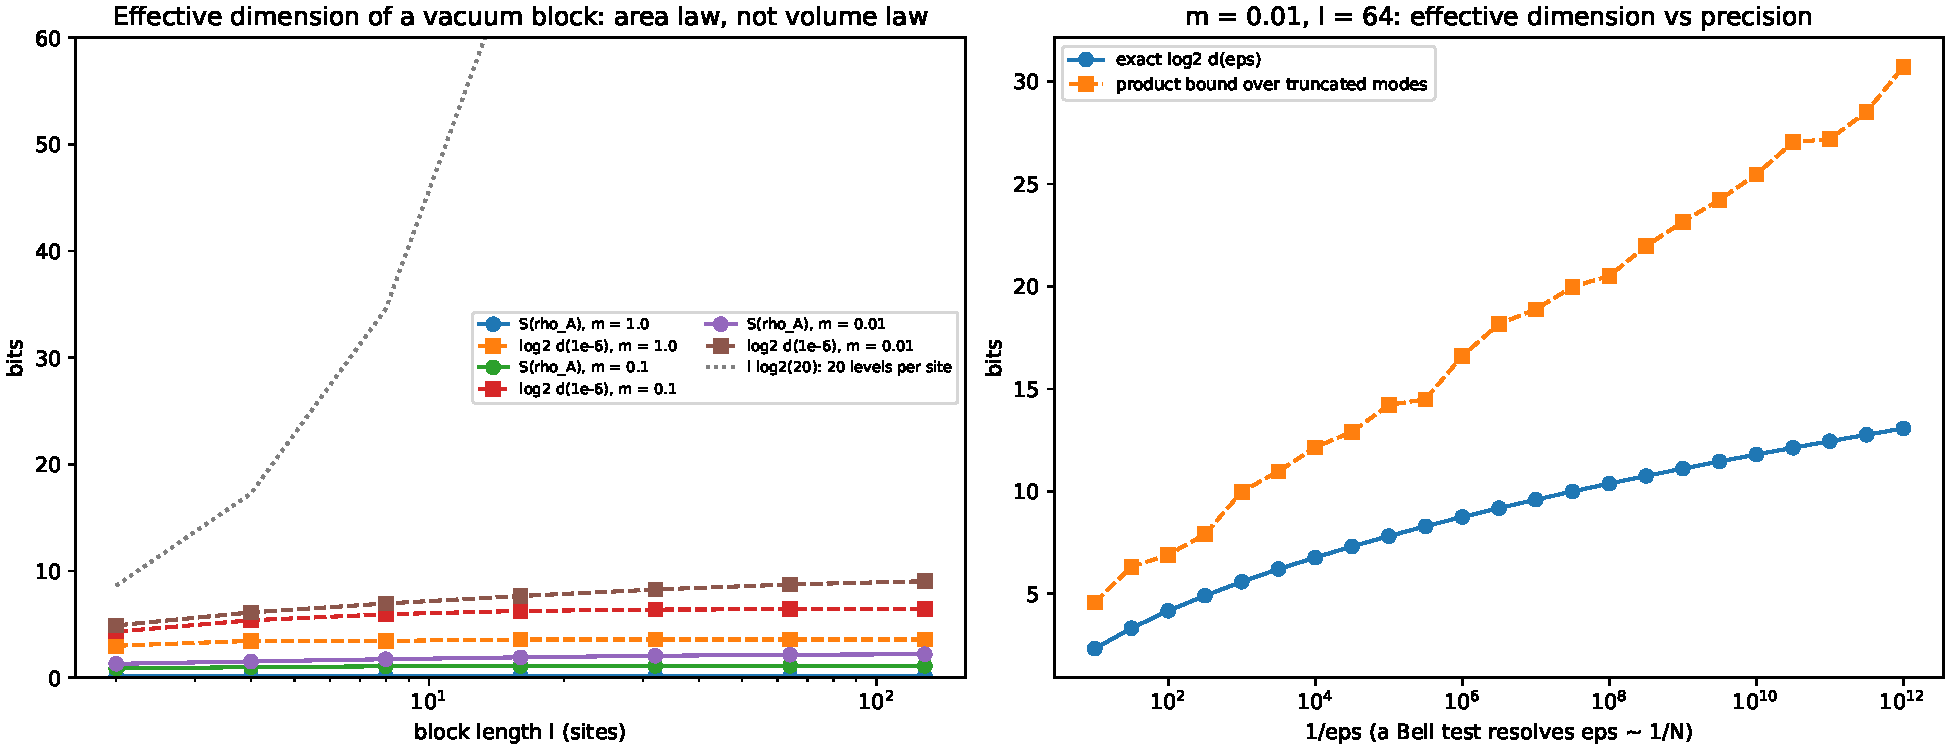
\includegraphics[width=\textwidth]{qft_effective_dimension.pdf}
\caption{\emph{Left:} entanglement entropy $S(\rho_A)$ (circles) and $\log_2d_{\rho_A}(10^{-6})$ (squares) of a block of $l$ sites in the
vacuum of the harmonic chain for $m=1,0.1,0.01$, compared with the naive count $l\log_220$. \emph{Right:} $\log_2d_{\rho_A}(\varepsilon)$
for $m=0.01$, $l=64$, together with the product bound of Proposition~\ref{prop:product}.}
\label{fig:main}
\end{figure}

\begin{table}[ht]
\centering
\caption{Entanglement entropy and effective dimension $\log_2d_{\rho_A}(\varepsilon)$, in bits, for blocks of the harmonic-chain
vacuum.}
\label{tab:dim}
\small
\begin{tabular}{rrrrrr}
\toprule
$m$ & $l$ & $S$ & $\varepsilon=10^{-2}$ & $10^{-4}$ & $10^{-6}$ \\
\midrule
1 & 128 & 0.161 & 1.00 & 2.58 & 3.58 \\
0.1 & 8 & 1.075 & 2.58 & 4.46 & 5.95 \\
0.1 & 128 & 1.111 & 2.58 & 4.86 & 6.43 \\
0.01 & 8 & 1.737 & 3.32 & 5.39 & 6.97 \\
0.01 & 32 & 2.062 & 3.91 & 6.43 & 8.28 \\
0.01 & 128 & 2.204 & 4.25 & 6.99 & 9.05 \\
\bottomrule
\end{tabular}
\end{table}

Table~\ref{tab:dim} and Figure~\ref{fig:main} show two features. First, the effective dimension follows the entanglement
entropy, an area law, and not the number of degrees of freedom. For $m=1$ and $m=0.1$ it saturates once the block exceeds the
correlation length. For $m=0.01$ it grows logarithmically, like the entropy of a nearly critical chain. At $l=128$ and
$\varepsilon=10^{-6}$ it is $9$ bits, while counting $20$ levels per site would give $553$ bits. Second, the dependence on precision is
weak. At $m=0.01$, $l=64$ ($S=2.16$ bits), $\log_2d(\varepsilon)$ grows from $2.3$ bits at $\varepsilon=10^{-1}$ to $13.1$ bits at $\varepsilon=10^{-12}$. The local slope
$\dd\log_2d/\dd\log_2(1/\varepsilon)$ falls from $0.60$ to $0.25$ at $\varepsilon\sim10^{-6}$ and to $0.19$ at $\varepsilon\sim10^{-12}$.

\begin{proposition}
\label{prop:product}
Let $\rho=\bigotimes_{k=1}^K\rho_{q_k}$ be a product of thermal modes with spectra $(1-q_k)q_k^n$. Then
\begin{equation}
d_\rho(\varepsilon)\le\prod_{k=1}^K\Bigl\lceil\frac{\ln(K/\varepsilon)}{\ln(1/q_k)}\Bigr\rceil=O\bigl((\ln1/\varepsilon)^K\bigr).
\end{equation}
\end{proposition}

\begin{proof}
Keep occupations $0,\dots,n_k-1$ of mode $k$ with $n_k=\lceil\ln(K/\varepsilon)/\ln(1/q_k)\rceil$. The discarded weight of mode $k$ is $q_k^{n_k}\le\varepsilon/K$,
so by the union bound the projector onto the kept product subspace captures weight at least $1-\varepsilon$. Its rank is $\prod_kn_k$.
\end{proof}

For a block of a regularised field the number of relevant modes is finite, so the certifiable dimension grows
polylogarithmically in the precision. By Proposition~\ref{prop:compress}, $N$ rounds resolve $\delta\sim N^{-1/2}$, i.e.\ $\varepsilon\sim1/N$, so the
certifiable number of bits grows only as $O(K\log\log N)$. The bound is loose by a factor of about two in our example
(Figure~\ref{fig:main}, right), but it captures the shape of the growth.

%=====================================================================
\section{Discussion}
\label{sec:discussion}

The companion paper~\cite{Chen2026_certify} left one way in which a finite experiment could certify an actual infinity:
a Bell violation in the gap between $\Cqa$ and $\Cqc$. For local measurements in relativistic QFT with the split property
or hyperfinite local algebras, this gap is unreachable (Corollary~\ref{cor:qft}). The same holds for the observer
algebra of semiclassical de Sitter gravity (Proposition~\ref{prop:dS}). Within these frameworks every Bell correlation
is approximable by finite-dimensional ones. The approximating dimension is set by the smooth max-entropy of the local
state. For the vacuum it follows an area law and grows only polylogarithmically with the precision.

Three caveats bound these conclusions. First, they concern local measurements in the sense of algebraic QFT. Measurements
that are not localised, or theories without the split property, for instance with too many local degrees of freedom,
are not covered. Second, the hyperfiniteness theorem of~\cite{BDF} assumes a scaling limit, and Proposition~\ref{prop:dS}
assumes injectivity of the static-patch QFT algebra. Third, Proposition~\ref{prop:product} is a statement about regularised
blocks. In the continuum the effective dimension depends on the size of the split gap, which acts as a cutoff, and
should be computed on the canonical splitting factor (Remark in Section~\ref{sec:effective}).

Together with~\cite{Chen2026_certify}, the result is a coherent picture. Physics routinely uses infinite-dimensional
Hilbert spaces and type III algebras. Yet the correlations that local measurements can produce in these frameworks
are reproduced, to any finite precision, by finite-dimensional models whose size is controlled by entanglement entropy.
In this sense, the actual infinity of quantum field theory is not empirically accessible through Bell experiments.

\section*{Data and code availability}
The script \texttt{qft\_effective\_dimension.py}, the data (CSV), the figure and the console output are available at
\url{https://github.com/Ruqing1963/qft-tsirelson-loophole} and archived under DOI \href{https://doi.org/\paperdoi}{\paperdoi}.

%=====================================================================
\begin{thebibliography}{99}\small
\bibitem{Haag} R.~Haag, \emph{Local Quantum Physics: Fields, Particles, Algebras}, 2nd ed., Springer, Berlin (1996).
\bibitem{ScholzWerner} V.~B.~Scholz, R.~F.~Werner, ``Tsirelson's problem'', arXiv:0812.4305 (2008).
\bibitem{Fritz} T.~Fritz, ``Tsirelson's problem and Kirchberg's conjecture'', Rev.\ Math.\ Phys.\ 24 (2012) 1250012, arXiv:1008.1168.
\bibitem{JungeEtAl} M.~Junge, M.~Navascu\'es, C.~Palazuelos, D.~P\'erez-Garc\'ia, V.~B.~Scholz, R.~F.~Werner, ``Connes' embedding problem and Tsirelson's problem'', J.\ Math.\ Phys.\ 52 (2011) 012102, arXiv:1008.1142.
\bibitem{MIPRE} Z.~Ji, A.~Natarajan, T.~Vidick, J.~Wright, H.~Yuen, ``MIP$^*$=RE'', arXiv:2001.04383 (2020).
\bibitem{Chen2026_certify} R.~Chen, ``Can finite experiments certify actual infinity? Dimension witnesses, Tsirelson's problem, and holographic resource bounds'' (2026), doi:10.5281/zenodo.23202129.
\bibitem{CabelloQuintinoKleinmann} A.~Cabello, M.~T.~Quintino, M.~Kleinmann, ``Possible consequences for physics of the negative resolution of Tsirelson's problem'', arXiv:2307.02920 (2023).
\bibitem{DoplicherLongo} S.~Doplicher, R.~Longo, ``Standard and split inclusions of von Neumann algebras'', Invent.\ Math.\ 75 (1984) 493--536.
\bibitem{BuchholzWichmann} D.~Buchholz, E.~H.~Wichmann, ``Causal independence and the energy-level density of states in local quantum field theory'', Commun.\ Math.\ Phys.\ 106 (1986) 321--344.
\bibitem{Haagerup} U.~Haagerup, ``Connes' bicentralizer problem and uniqueness of the injective factor of type III$_1$'', Acta Math.\ 158 (1987) 95--148.
\bibitem{BDF} D.~Buchholz, C.~D'Antoni, K.~Fredenhagen, ``The universal structure of local algebras'', Commun.\ Math.\ Phys.\ 111 (1987) 123--135.
\bibitem{Connes} A.~Connes, ``Classification of injective factors. Cases II$_1$, II$_\infty$, III$_\lambda$, $\lambda\ne1$'', Ann.\ Math.\ 104 (1976) 73--115.
\bibitem{EffrosLance} E.~G.~Effros, E.~C.~Lance, ``Tensor products of operator algebras'', Adv.\ Math.\ 25 (1977) 1--34.
\bibitem{Paulsen} V.~I.~Paulsen, \emph{Completely Bounded Maps and Operator Algebras}, Cambridge University Press (2002).
\bibitem{CLPW} V.~Chandrasekaran, R.~Longo, G.~Penington, E.~Witten, ``An algebra of observables for de Sitter space'', JHEP 02 (2023) 082, arXiv:2206.10780.
\bibitem{BrownOzawa} N.~P.~Brown, N.~Ozawa, \emph{C$^*$-Algebras and Finite-Dimensional Approximations}, Graduate Studies in Mathematics 88, American Mathematical Society (2008).
\bibitem{RennerWolf} R.~Renner, S.~Wolf, ``Smooth R\'enyi entropy and applications'', Proc.\ IEEE Int.\ Symp.\ Inf.\ Theory (2004) 233.
\bibitem{Winter} A.~Winter, ``Coding theorem and strong converse for quantum channels'', IEEE Trans.\ Inf.\ Theory 45 (1999) 2481--2485.
\bibitem{LongoXu} R.~Longo, F.~Xu, ``Von Neumann entropy in QFT'', Commun.\ Math.\ Phys.\ 381 (2021) 1031--1054, arXiv:1911.09390.
\bibitem{PanebiancoWegener} L.~Panebianco, B.~Wegener, ``Entanglement entropy in CFT and modular nuclearity'', arXiv:2108.09074.
\bibitem{DuttaFaulkner} S.~Dutta, T.~Faulkner, ``A canonical purification for the entanglement wedge cross-section'', JHEP 03 (2021) 178, arXiv:1905.00577.
\bibitem{BuenoCasini} P.~Bueno, H.~Casini, ``Reflected entropy, symmetries and free fermions'', JHEP 05 (2020) 103, arXiv:2003.09546.
\bibitem{PeschelEisler} I.~Peschel, V.~Eisler, ``Reduced density matrices and entanglement entropy in free lattice models'', J.\ Phys.\ A 42 (2009) 504003, arXiv:0906.1663.
\bibitem{AudenaertEtAl} K.~Audenaert, J.~Eisert, M.~B.~Plenio, R.~F.~Werner, ``Entanglement properties of the harmonic chain'', Phys.\ Rev.\ A 66 (2002) 042327, arXiv:quant-ph/0205025.
\end{thebibliography}

\end{document}
